\section{Network II - Non-tumour split}


\subsection{Communities} \label{ap:N_II:coms}

\subsubsection{Community 25}

\begin{figure}[H]    
    \centering
    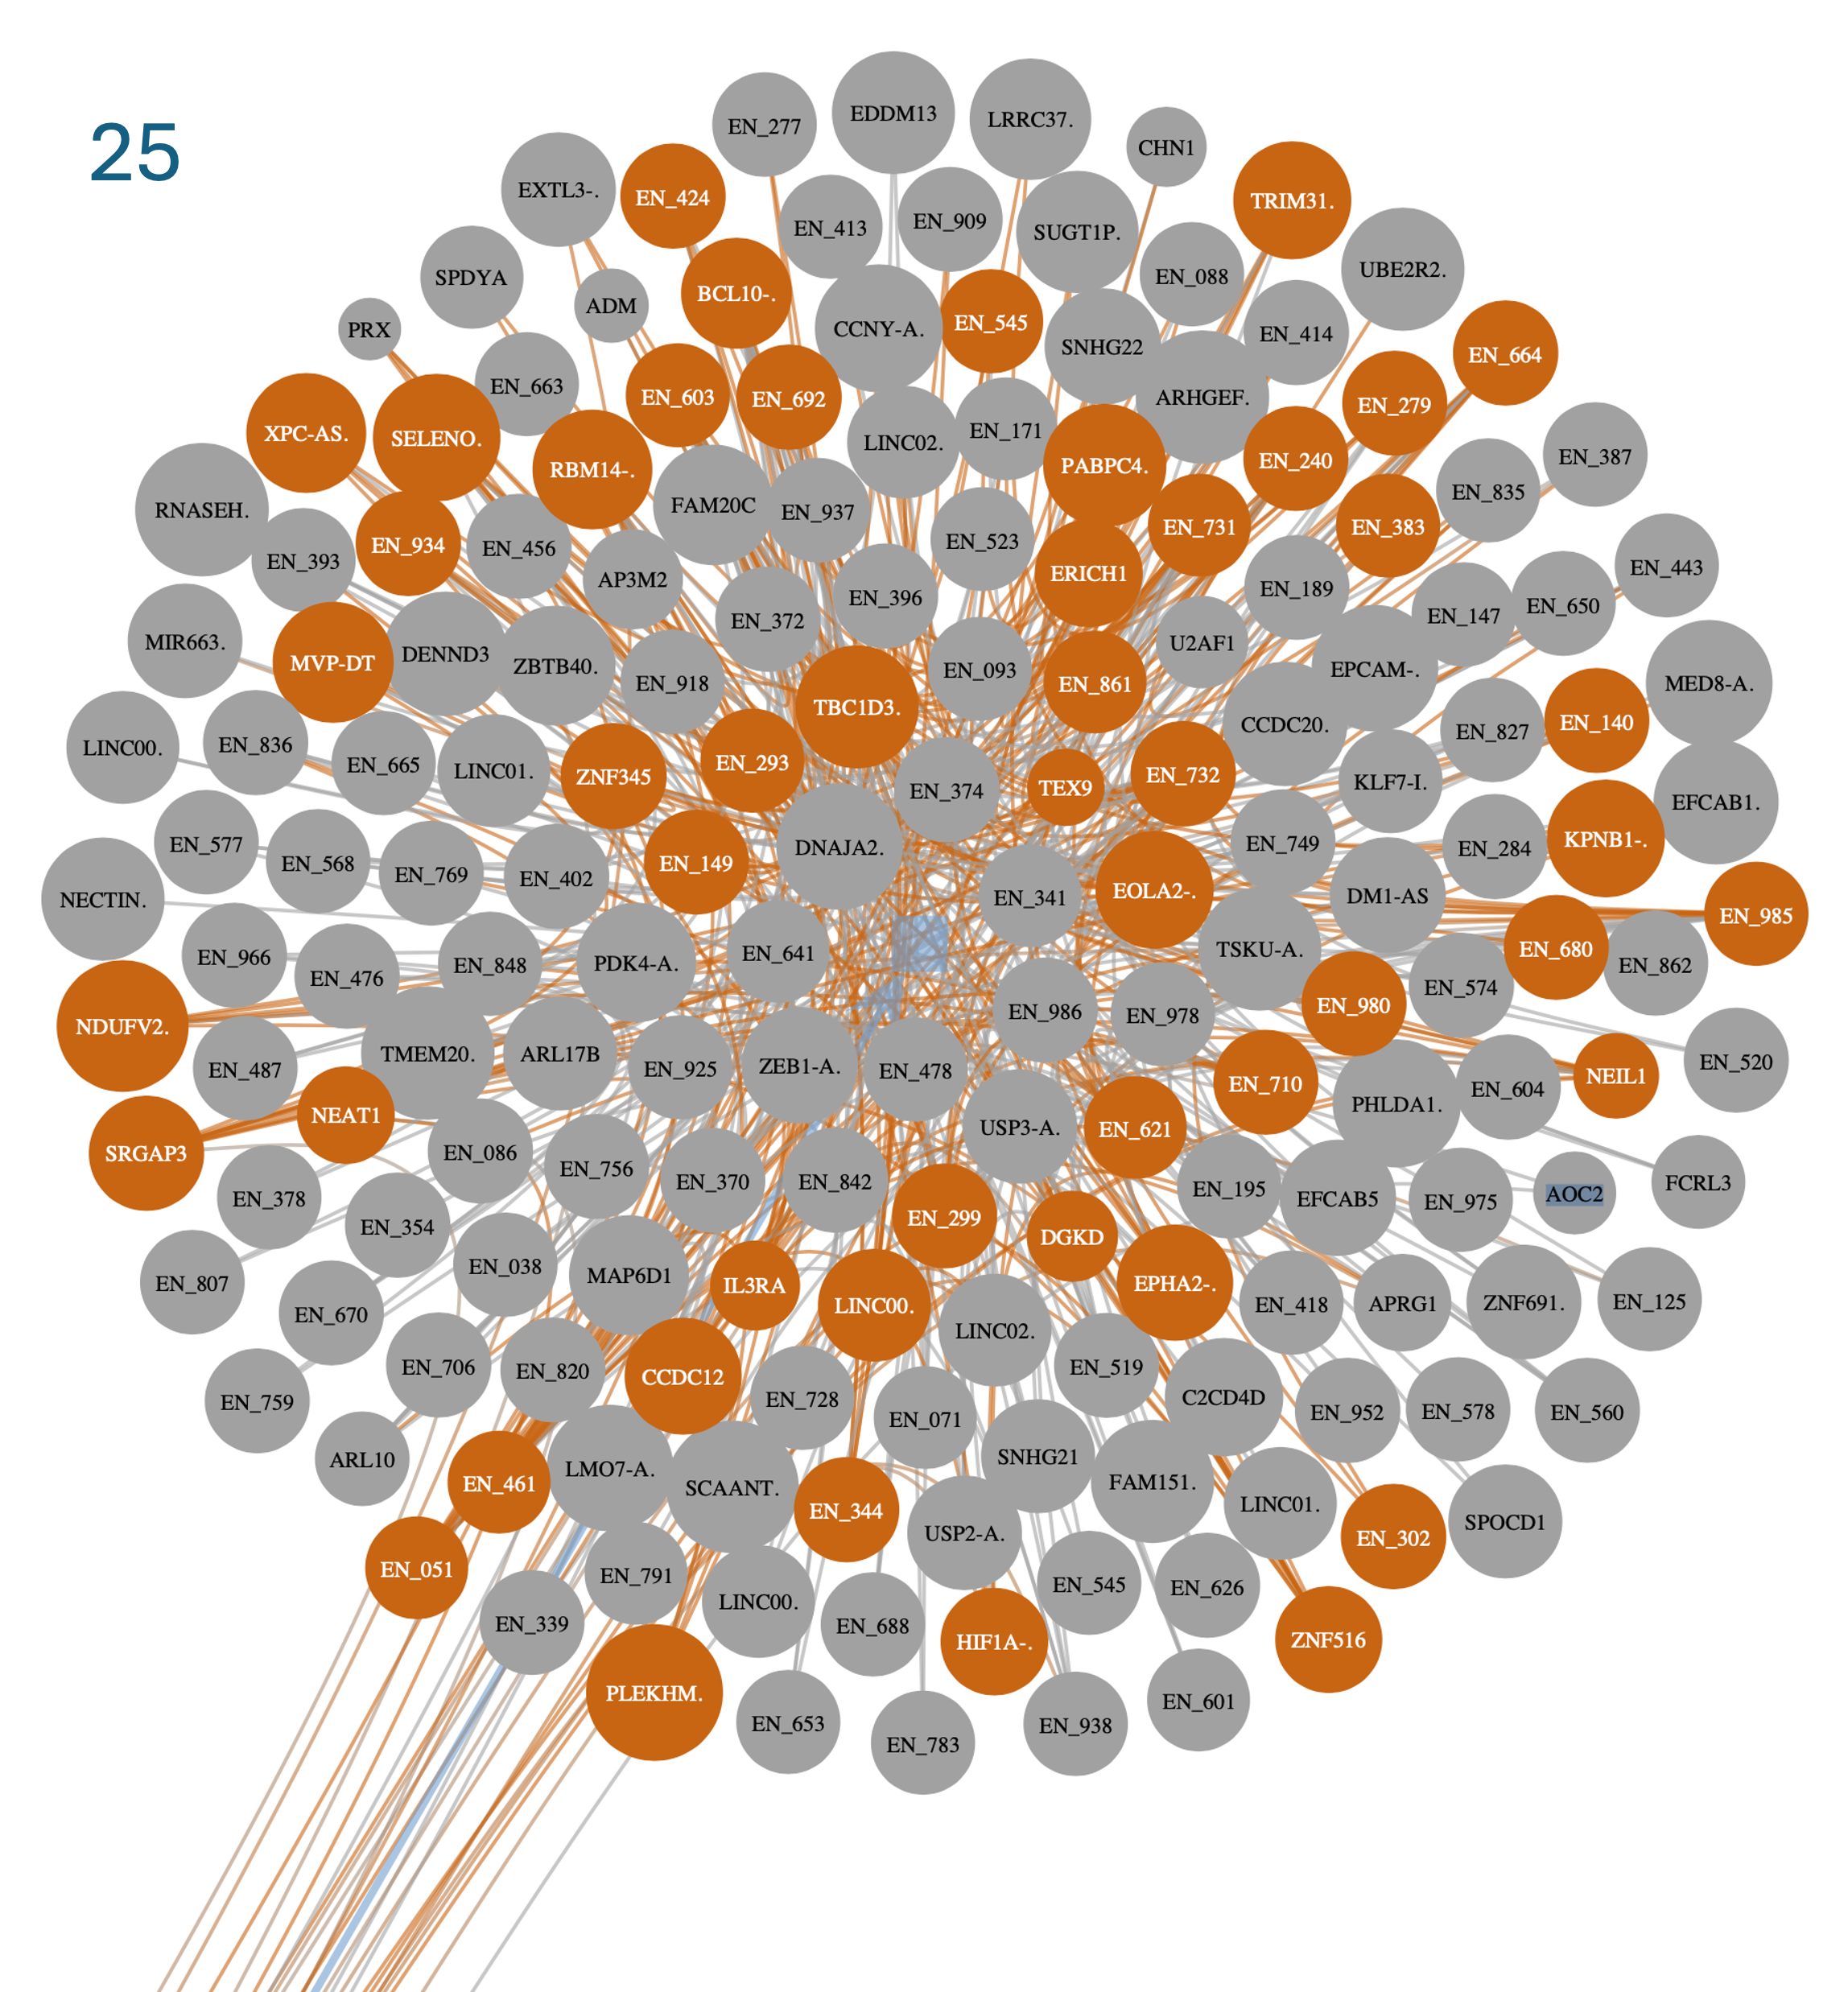
\includegraphics[width=1.0\textwidth,height=1.0\textheight,keepaspectratio]{Sections/Network_II/resources/non_tum/25_com.png}
    \caption{Community 25 from the standard network generated from 5000 genes, no weight modifier and to which the \acrshort{hsbm} was applied. The community contains 180 genes from which 50 with the highest ModCon score are highlighted in orange. To aid the visualisation some of the genes were trim, for the ones with longer names the first 5 letters were kept while for 'ENSG...' like nodes the "EN\_" and the last 3 digits were kept. See \cref{s:N_II:comm_charact} for more details. }
    \label{fig:ap:com_29}
\end{figure}


\subsubsection{Community 29}

\begin{figure}[H]    
    \centering
    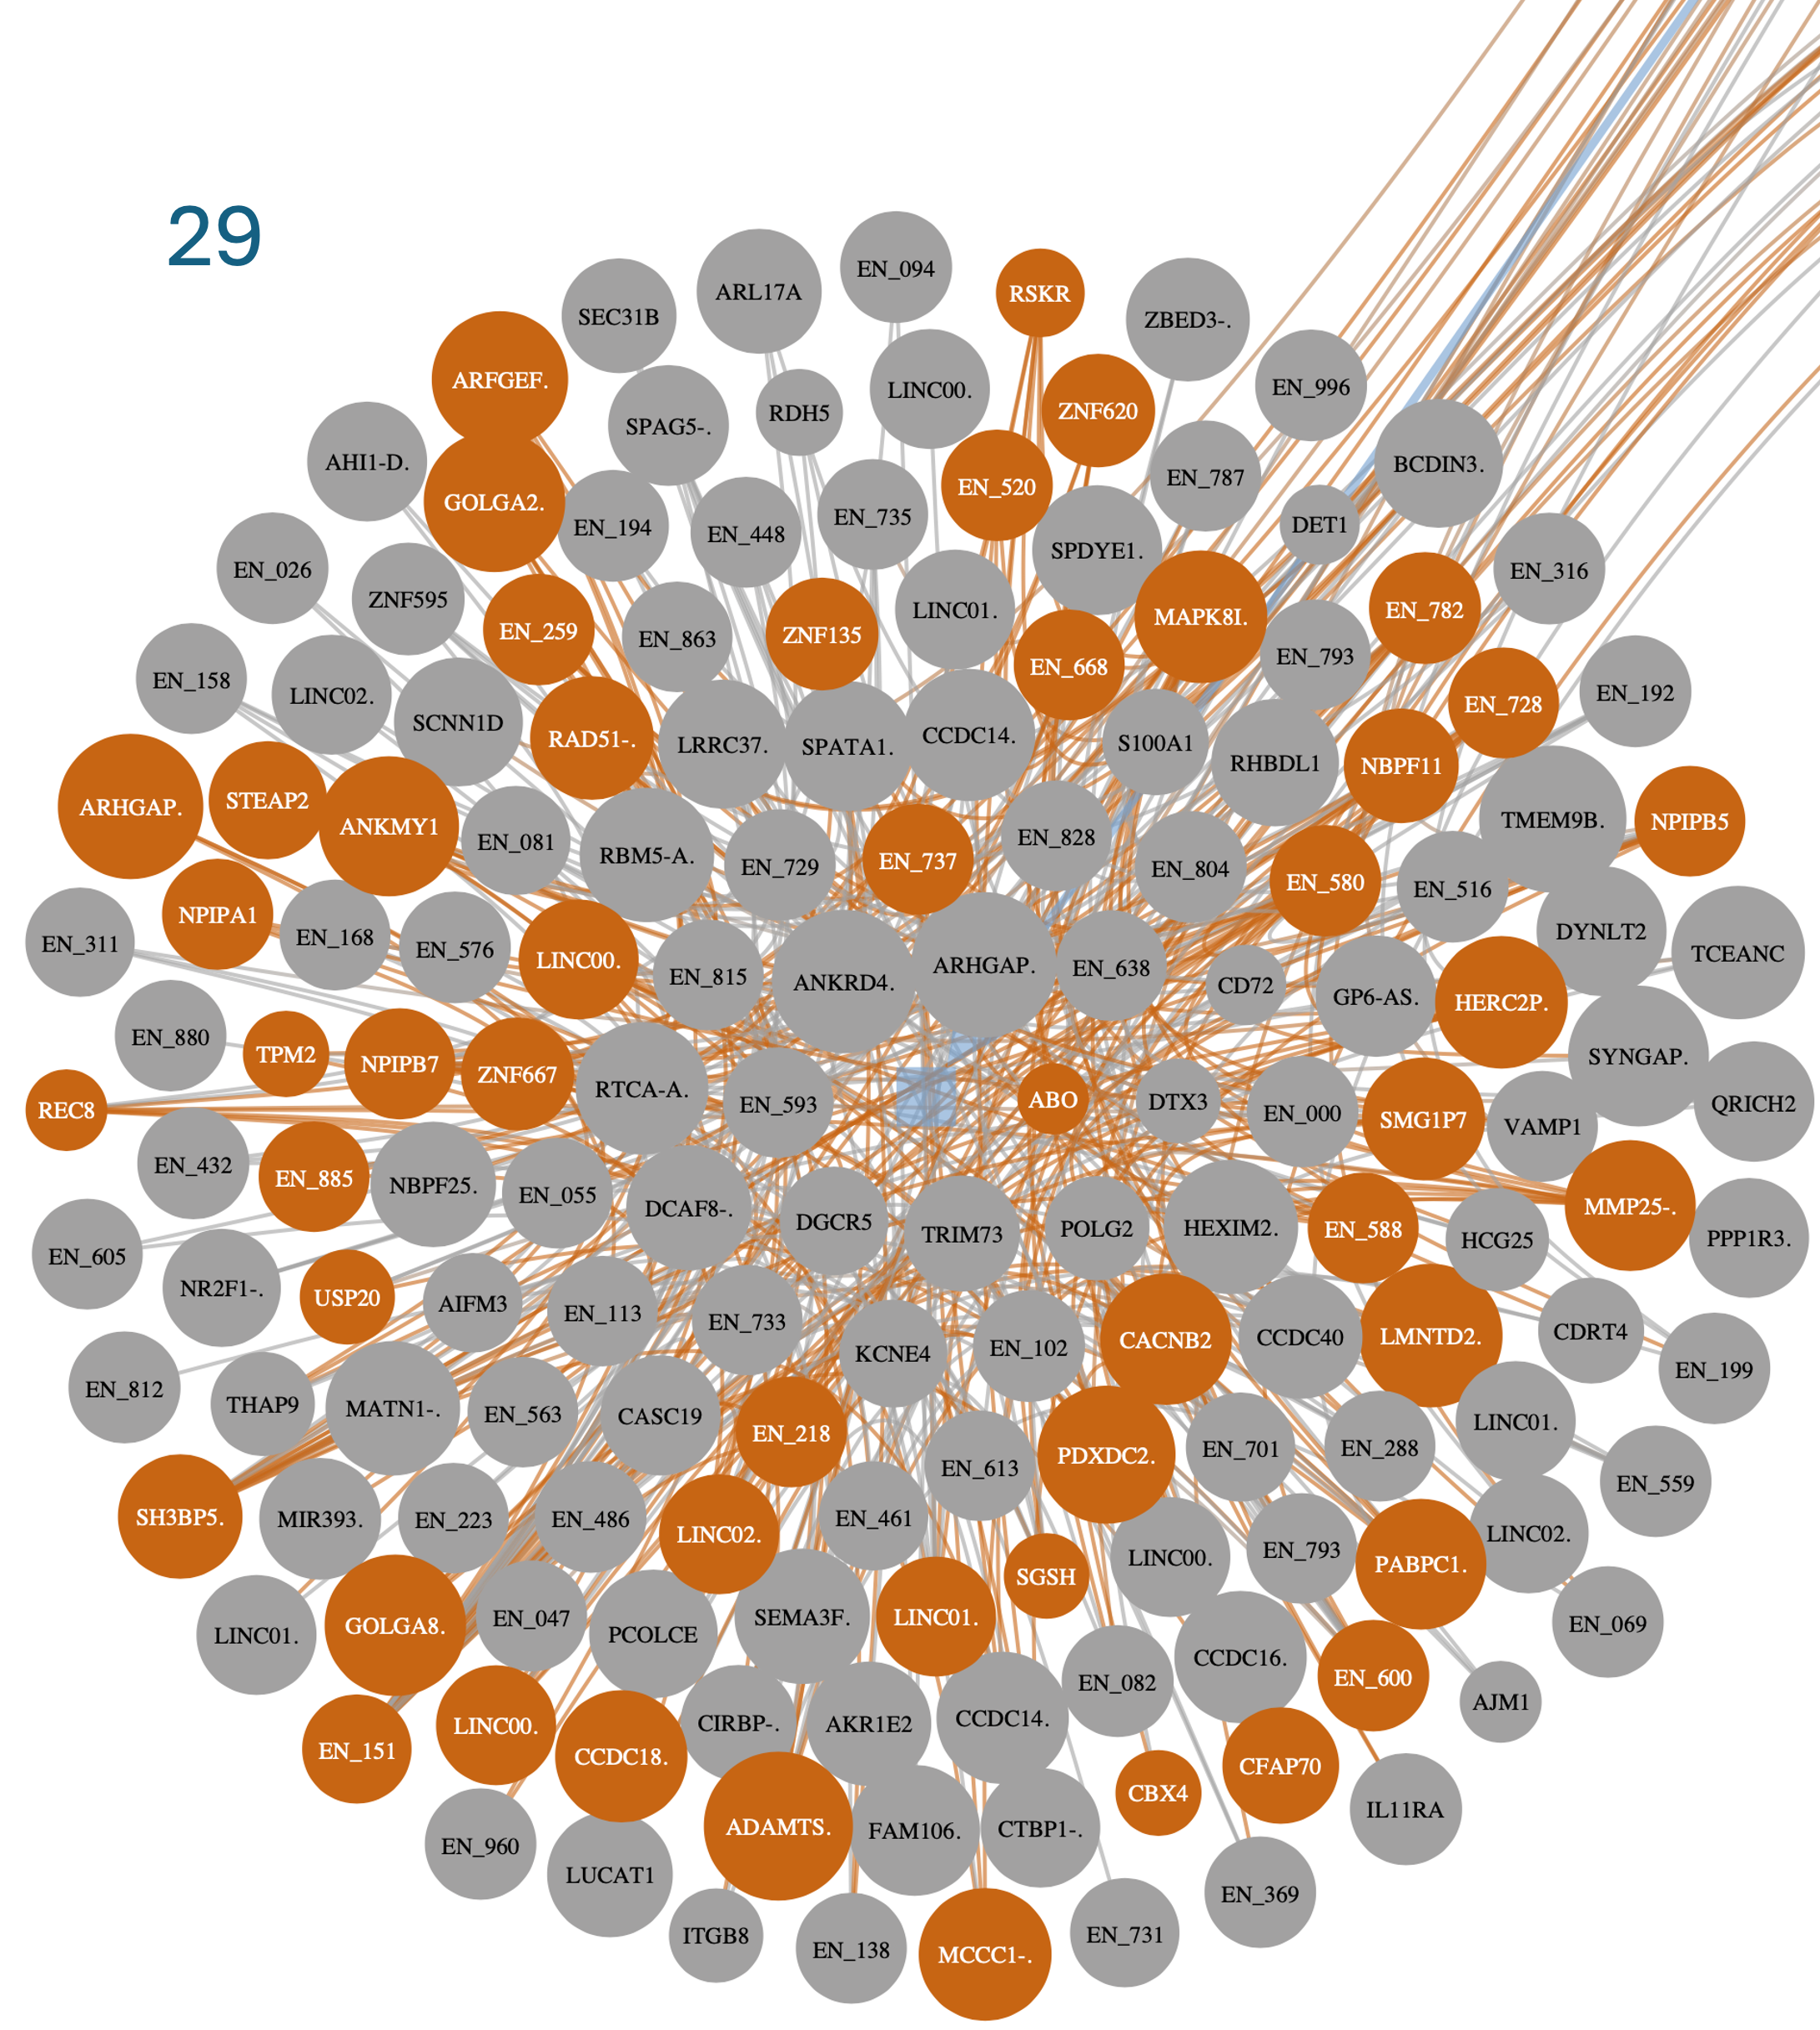
\includegraphics[width=1.0\textwidth,height=1.0\textheight,keepaspectratio]{Sections/Network_II/resources/non_tum/29_com.png}
    \caption{Community 25 from the standard network generated from 5000 genes, no weight modifier and to which the \acrshort{hsbm} was applied. The community contains 164 genes from which 50 with the highest ModCon score are highlighted in orange. To aid the visualisation some of the genes were trim, for the ones with longer names the first 5 letters were kept while for 'ENSG...' like nodes the "EN\_" and the last 3 digits were kept.  See \cref{s:N_II:comm_charact} for more details. }
    \label{fig:ap:com_29}
\end{figure}
